%!TEX root = ../book.tex
\section{Inverse Kinematics}\label{sec:kinematics:ik}

The forward kinematics of a system are computed by means of a transformation matrix from the base of a manipulator (or a corner of the room) to the end-effector of a manipulator (or a mobile robot).
As such, they are an exact description of the pose of the robot and they fully characterize its kinematic state.
Inverse Kinematics deal with the opposite problem, that is how to find a joint configuration that leads to a desired pose at the end effector.
To achieve this goal, we will need to solve the forward kinematics equations for joint angles as a function of the desired pose.
With reference to \cref{eq:kinematics:forward}, inverse kinematics aims to solve the following:
\begin{equation}\label{eq:kinematics:inverse}
q = f^{-1} (r)\ , \qquad f^{-1} : \mathbb{R}^m \rightarrow \mathbb{R}^n \ ,
\end{equation}
with a notation similar to \cref{eq:kinematics:forward}.
For a mobile robot, we can do this only for velocities in the local coordinate system, and need more sophisticated methods to calculate appropriate trajectories for the robot.

\subsection{Solvability}

\cref{eq:kinematics:inverse} is the inverted version of \cref{eq:kinematics:forward}, and as such is heavily non-linear.
Therefore, it makes sense to briefly think about whether we can solve it at all for specific parameters before trying.
Here, the workspace of a robot becomes important. The workspace is the sub-space that can be reached by the robot in any orientation.
Clearly, there will be no solutions for the inverse kinematic problem outside of the workspace of the robot.

A second question to ask is how many solutions we actually expect and what it means to have multiple solutions \textsl{geometrically}.
Multiple solutions to achieve a desired pose correspond to multiple ways in which a robot can reach a target.
For example a three-link arm that wants to reach a point that can be reached without fully extending all links (leading to a single solution), can do this by folding its links in a concave and a convex fashion.
How many solutions there are for a given mechanism and pose quickly becomes non-intuitive.
For example, a 6-DOF arm can reach certain points with up to $16$ different configurations!

\subsection{Inverse Kinematics of a Simple Manipulator Arm}\label{sec:kinematics:inverse:arm}

We will now look at the inverse kinematics of the $2-$link arm that we introduced in \cref{fig:fwk2dofarm}. We need to solve the equations determining the robot's forward kinematics by solving for $\alpha$ and $ \beta$.
This is tricky, however, as we have to deal with complicated trigonometric expressions.

To get an intuition, assume there to be only one link, $l_1$.  Solving (\ref{eq:cosxl1}) for $\alpha$ yields to two distinct solutions:
\td{Nikolaus: Can't we just say +-cos here?}
\begin{equation}
\alpha = \left[\cos^{-1}\frac{x_1}{l_1},-\cos^{-1}\frac{x_1}{l_1}\right]\ ,
\end{equation}
as cosine is symmetric for positive and negative values.
Indeed, for any possible position on the $x-$axis ranging from $-l_1$ to $l_1$, there exist two solutions: the first one with the arm above the table, and the other one with the arm below it.
At the extremes of the workspace, both solutions are the same.

%\begin{verbatim}
%sol = Solve[Sin[a + b] + Sin[a] == y
%              && Cos[a + b] + Cos[a] == x,
%             {a, b}];
%min = sol /. {x -> 1, y -> 1}
%\end{verbatim}

Solving for both degrees of freedom actually yields eight solutions, of which only two are feasible:
\td{Nikolaus: where are the two solutions in the equations below and why is there an arrow ?}

\begin{eqnarray}
\alpha &\rightarrow& \cos^{-1}\left(\frac{x^2 y + y^3 - \sqrt{4 x^4 - x^6 + 4 x^2 y^2 - 2 x^4 y^2 - x^2 y^4}}{2 (x^2 + y^2)}\right) \nonumber \\
\beta &\rightarrow& -\cos^{-1}\left( \frac{1}{2}(-2+x^2+y^2) \right)
\end{eqnarray}
1
What will drastically simplify this problem, is to not only specify the desired position, but also the orientation $\theta$ of the end-effector. In this case, a desired pose can be specified by
\begin{equation}
\left[
\begin{array}{cccc}
cos\theta & -sin\theta & 0 & x\\
sin\theta & cos\theta & 0 & y\\
0 & 0 & 1 & 0\\
0 & 0 & 0 & 1
\end{array}
\right]
\end{equation}
A solution can now be found by simply equating the individual entries of the transformation (\ref{eq:2armtrans}) with those of the desired pose. Specifically, we can observe:
\begin{eqnarray}
cos\theta &=& cos(\alpha+\beta)\\
\nonumber
x &=& \cos_{\alpha\beta}l_2+\cos\alpha l_1\\
\nonumber
y &=& \sin_{\alpha\beta}l_2+\sin\alpha l_1
\end{eqnarray}
These can be reduced to
\begin{eqnarray}
\theta &=& \alpha + \beta \nonumber \\
\cos\alpha &=& \frac{\cos_{\alpha\beta}l_2-x}{l_1}=\frac{\cos\theta l_2-x}{l_1} \\
\sin\alpha &=& \frac{\sin_{\alpha\beta}l_2-y}{l_1}=\frac{\sin\theta l_2-y}{l_1} \nonumber
\end{eqnarray}
Providing the orientation of the robot in addition to the desired position therefore allows solving for $\alpha$ and $\beta$ just as a function of $x$, $y$ and $\theta$.

The main issue with the geometric approach detailed above is that it does not scale easily with an increase of DoF at the joints, and and it quickly becomes unhandy with more dimensions.
For higher-DoF platforms, we can calculate a \textsl{numerical solution} using an approach that we will later see is very similar to path planning in mobile robotics.
To this end, we will first calculate a measure of error between the current solution and the desired one, and then optimize the joint configuration so as to minimize such error.
In our example, the measure of error is the distance between the current end-effector pose as given by the forward kinematics equations in \cref{eq:fwk2dofarm} and the desired solution $[x,y]$ in configuration space, i.e.:
% To do this, you need to solve the forward kinematics for every point in configuration space and use the Euclidean distance to the desired target as height.
\td{nikolaus: why there are no $l_1$ and $l_2$ in the eq below?}
\begin{equation}\label{eq:kinematics:inverse:numerical}
f_{x,y}(\alpha,\beta)=\sqrt{\left(\sin_{\alpha\beta} + \sin_\alpha - y\right)^2 + \left(\cos_{\alpha\beta}+\cos_\alpha - x\right)^2}
\end{equation}
\cref{eq:kinematics:inverse:numerical} is a 3D functional and can be plotted as a function of $\alpha$ and $\beta$, our joint-space variables.
% This is plotted for $\alpha=[-\pi/2,\pi/2]$ and $\beta=[-\pi,\pi]$ and $x=1$, $y=1$ in Figure~\ref{fig:inversekinematics}.
As shown in \cref{fig:inversekinematics}, this function has a minima, in this case zero, for values of $\alpha$ and $\beta$ that bring the manipulator to $(1,1)$. These values are $(\alpha \rightarrow 0, b \rightarrow -\frac{\pi}{2})$ and $(\alpha \rightarrow -\frac{\pi}{2}, b \rightarrow \frac{\pi}{2})$.

\begin{figure}
    \centering
        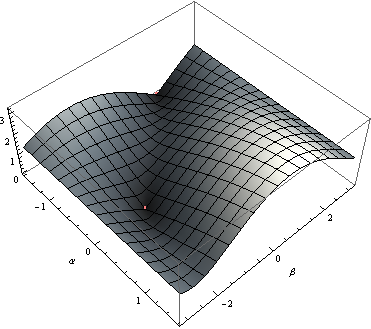
\includegraphics[width=0.8\textwidth]{figs/inversekinematics}
    \caption{Distance to $(x=1,y=1)$ over the configuration space of a two-arm manipulator. Minima corresponds to exact inverse kinematic solutions.}
    \label{fig:inversekinematics}
\end{figure}

You can now think about inverse kinematics as a path finding problem from anywhere in the configuration space to the nearest minima. A formal approach to doing this will be discussed in \cref{sec:kinematics:inverse:feedbackcontrol}. How to find shortest paths in space, that is finding the shortest route for a robot to get from A to B will be a subject of chapter~\ref{chap:pathplanning}.

\subsection{Inverse Kinematics of Mobile Robots}\label{sec:kinematics:ik:mobile}

There is no unique relationship between the amount of rotation of a robot's individual wheels and its position in space; however, for simple holonomic platforms such as a robot on a track, we will treat the inverse kinematics problem at first only for the velocities of the local robot coordinate frame.
%
Let's first establish how to calculate the necessary speed of the robot's center given a desired speed $ \dot{\xi_I}$ in world coordinates. We can transform the expression $ \dot{\xi_I}=T(\theta)\dot{\xi_R}$ by multiplying both sides with the inverse of $ T(\theta)$:

\begin{equation}\label{eq:mbik}
T^{-1}(\theta)\dot{\xi_I}=T^{-1}(\theta)T(\theta)\dot{\xi_R}
\end{equation}
which leads to $ \dot{\xi_R}=T^{-1}(\theta)\dot{\xi_I}$. Here

\begin{equation}
T^{-1}=\left[\begin{array}{ccc}cos \theta & sin \theta & 0 \\ -sin \theta & cos \theta & 0 \\ 0 & 0 & 1\end{array}\right]
\end{equation}
which can be computed by performing the matrix inversion or by deriving the trigonometric relationships from the drawing.  Similarly to \cref{sec:kinematics:inverse:arm}, we can now solve \cref{eq:kinematics:forward:mobile}
% \begin{equation}
% \left[\begin{array}{c} \dot{x_R}\\\dot{y_R}\\\dot{\theta}\end{array}\right]=\left[\begin{array}{c}\frac{r\dot{\phi_l}}{2}+\frac{r\dot{\phi_r}}{2}\\0\\\frac{\dot{\phi_r} r}{d}-\frac{\dot{\phi_l} r}{d}\end{array}\right]
% \end{equation}
for $ \phi_l$, $ \phi_r$:
\begin{eqnarray}
\dot{\phi}_l &= (2\dot{x}_R - \dot{\theta}d)/2r\\
\nonumber
\dot{\phi}_r &= (2\dot{x}_R + \dot{\theta}d)/2r
\end{eqnarray}
allowing us to calculate the robot's wheel speed as a function of a desired $\dot{x}_R$ and $\dot{\theta}$, which can be calculated using (\ref{eq:mbik}).

Note that this approach does not allow us to deal with $\dot{y}_R \neq 0$, which might result from a desired speed in the inertial frame. Non-zero values for translation in y-direction are simply ignored by the inverse kinematic solution, and driving toward a specific point either requires feedback control (Section~\ref{sec:kinematics:ik:invjac}) or path planning (Chapter~\ref{chap:pathplanning}).

\section{Inverse Kinematics using Feedback Control}\label{sec:kinematics:inverse:feedbackcontrol}

Solving the inverse kinematic problem for non-holonomic mobile robots requires us to find a sequence of actuation commands.
One way of doing this is to employ \emph{feedback control}\index{Feedback Control}.
In a nutshell, feedback control uses the error between actual and desired position to calculate a trajectory that drives the robot a little closer to its desired pose. The process is then repeated until the error is marginally small.
This approach can not only be used for mobile robots, but also for manipulator arms with kinematics that are too complicated to solve analytically.

\subsection{Feedback control for mobile robots}\label{sec:fbmobile}

Assume the robot's position given by $x_r, y_r$ and $\theta_r$ and the desired pose as $x_g, y_g$ and $\theta_g$---with the subscript $g$ indicating ``goal''.
We can now calculate the error in the desired pose by:
\begin{eqnarray}
\rho  &=& \sqrt{(x_r-x_g)^2+(y_r-y_g)^2} \nonumber \\
\alpha&=& \tan^{-1}{\frac{y_g-y_r}{x_g-x_r}}-\theta_r \\
\eta  &=& \theta_g-\theta_r\ , \nonumber
\end{eqnarray}
which is illustrated in Figure~\ref{fig:trajectorygen}.
These errors can be converted directly into robot's speeds, for example using a simple proportional controller with gains $p_1$, $p_2$ and $p_3$:
\begin{eqnarray}
\dot{x} &=& p_1 \rho\\
\dot{\theta} &=& p_2 \alpha + p_3 \eta
\end{eqnarray}
which will let the robot drive in a curve until it reaches the desired pose.

\begin{figure}
    \centering
    % 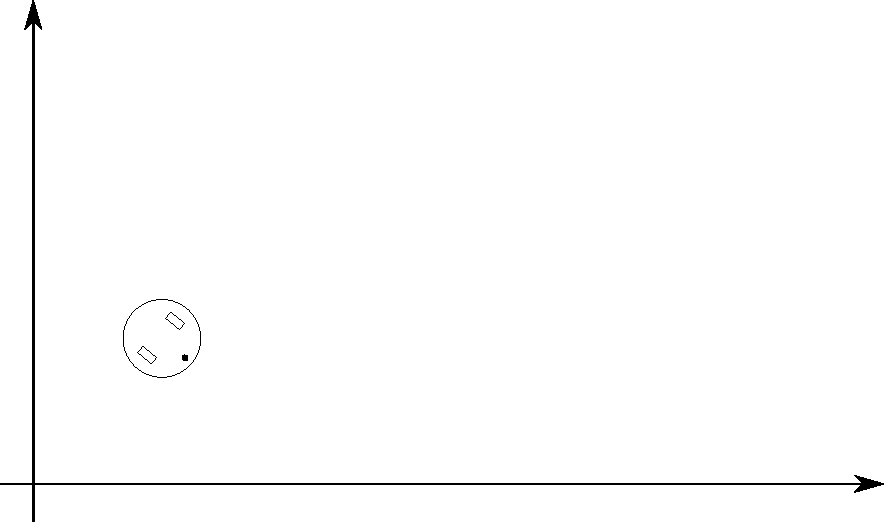
\includegraphics[width=\textwidth]{figs/trajectorygen.png}
    \def\svgwidth{\textwidth}
    \import{./figs/}{trajectorygen.pdf_tex}
    \caption{Difference in desired and actual pose as a function of distance $\rho$, bearing $\alpha$ and heading $\eta$.}
    \label{fig:trajectorygen}
\end{figure}


\subsection{Inverse Jacobian Technique}\label{sec:kinematics:ik:invjac}

The two-link arm in Figure~\ref{fig:fwk2dofarm} involved only two free parameters, but was already pretty complex to solve analytically if the end-effector pose was not specified.
One can imagine that things become very hard with more degrees of freedom or more complex geometries (mechanisms in which some axes intersect are simpler to solve than others, for example).
Fortunately, there are simple numerical techniques that work reasonably well in such situations.
One of them is known as the \emph{Inverse Jacobian}\index{Inverse Jacobian} technique.

As we can easily calculate the resulting pose for every possible joint angle combination using the forward kinematic equations, we can calculate the error between desired and actual pose.
This error actually provides us with a direction of motion that the end-effector needs to move toward so as to minimize such error.
As we only need to move tiny bits at a time and can then re-calculate the error, this is an attractive method to generate a trajectory that moves the arm to where we want it go and thereby solves the inverse kinematics problem.

In order to do this, we need an expression that relates the desired speed of the robot's end-effector, i.e. the direction in which we want to move, to the speed at which we need to change our joints.
This is known as \emph{Differential Kinematics}\index{Differential Kinematics}, as we are operating in the space of velocities, which are the derivative of positions.
Let the translational speed of a robot be given by:
\begin{equation}
v=\left[\begin{array}{c}
\dot{x}\\
\dot{y}\\
\dot{z}
\end{array}
\right].
\end{equation}
As the robot can potentially not only translate, but also rotate, we also need to specify its angular velocity. Let these velocities be given as a vector
\begin{equation}
\omega=\left[\begin{array}{c}
\omega_x\\
\omega_y\\
\omega_z
\end{array}
\right].
\end{equation}
We can now write translational and rotational velocities in a $6\times1$ vector as $\nu = [v \ \omega]^T$.
This notation is also called a \emph{velocity twist}.\index{Twist (velocity)}\index{Velocity Twist} %By convention, the speed of rotation is given by the magnitude (or length) of this vector.
Let the joint angles/positions be $q=[q_1, \ldots, q_n]^T$, and the set of joint speeds be $\dot{q}=[\dot{q}_1, \ldots, \dot{q}_n]^T$.
\td{I changed from $j$ to $q$ since $q$ is what everybody uses. I also changed a lot of the stuff below because it was confusing. Nikolaus please ack that you are aware of this.}
%
We now want to compute the differential kinematics version of \cref{eq:kinematics:forward}, which relates end-effector velocities $[v \ \omega]^T$ and joint velocities $\dot{q}$. In this case, it is given by:
\begin{equation}\label{eq:kinematics:diff:short}
\nu = [v \quad \omega]^T=J\cdot [\dot{q}_1,\ldots,\dot{q}_n]^T = J \cdot \dot{q}
\end{equation}
$J$ is known as the \emph{Jacobian matrix} \index{Jacobian Matrix} and contains all the partial derivatives of $f$ that relate every joint angle to every velocity. In practice, $J$ looks like:

\begin{equation}\label{eq:kinematics:diff}
\nu = \left[\begin{array}{c}v\\\omega\end{array}\right]=
\left[\begin{array}{c}\dot{x}\\
\dot{y}\\
\dot{z}\\
\omega_x\\
\omega_y\\
\omega_z\end{array}\right]=
\left[\begin{array}{cccc}\frac{\partial{x}}{\partial{q_1}} & \frac{\partial{x}}{\partial{q_2}} & \ldots & \frac{\partial{x}}{\partial{q_n}}\\\frac{\partial{y}}{\partial{q_1}} & \frac{\partial{y}}{\partial{q_2}} & \ldots & \frac{\partial{y}}{\partial{q_n}}\\\vdots & \vdots & \vdots & \vdots\\\frac{\partial{\omega_z}}{\partial{q_1}} & \frac{\partial{\omega_z}}{\partial{q_2}} & \ldots & \frac{\partial{\omega_z}}{\partial{q_n}}\end{array}\right]\left[\begin{array}{c}q_1\\\vdots\\q_n\end{array}\right] = J \cdot \dot{q}
\end{equation}

This notation is important as it tells us how small changes in joint space will affect the end-effector's position in cartesian space. Better yet, the forward kinematics of a mechanism can always be calculated, as well as their analytical derivatives, allowing us to calculate numerical values for the entries of matrix $J$ for every possible joint angle/position.

It would now be desirable to just invert $J$ in order to calculate the necessary joint speeds for every desired end-effector speeds---a problem known as \emph{Inverse Differential Kinematics}\index{Inverse Differential Kinematics}. Unfortunately, as any matrix $J$ is only invertible if the number of degrees of freedom in joint space $n$ equals the number of degrees of freedom in task space $m$, so that $ J$ is quadratic and has full rank.
In the case above, the velocity wrench $[v \ \omega]^T$ is $6-$dimensional, and this means that $n$ should be equal to $6$: therefore, inversion of $J$ is only possible if the robot under consideration is equipped with exactly $6$ actuators/joints.
If this is not the case, we can use the pseudo-inverse computation:
\begin{equation}
J^+=\frac{J^T}{JJ^T}=J^T(JJ^T)^{-1}
\end{equation}
As you can see, $J^T$ cancels from the equation leaving $1/J$, while being applicable to non-quadratic matrices.
We can now write a simple feedback controller that drives our error $e$ as the difference between desired and actual position to zero:
\begin{equation}
\Delta{q}=-J^+e
\end{equation}
That is, we move each joint a tiny bit into the direction that minimizes our error $e$.
It can be easily seen that the joint speeds are only zero if $e$ has become zero.

This solution might or might not be numerically stable, depending on the current joint values. If the inverse of $J$ is mathematically not feasible, we speak of a \emph{singularity}\index{Singularity} of the mechanism. This happens for example when two joint axes line up, therefore effectively removing a degree of freedom from the mechanism, or at the boundary of the workspace. As it happens very often in robotics, the concept of singularity has both a strong methematical justification (the joint configuration is such that the Jacobian is not full rank any more), and a direct physical consequence: singularity configurations are to be avoided as no solution for the inverse differential kinematics problem exist and the robot might become unsafe to operate.
In a singularity, the solution to $ J^+$ ``explodes'' and joint speeds go to infinity. In order to work around this, we can introduce damping to the controller.

In this case, we do not only minimize the error, but also the joint velocities. The minimization problem then becomes:
\begin{equation}
\|J\Delta q-e\|+\lambda^2\|\Delta q\|^2
\end{equation}
where $\lambda$ is some constant. One can show that the resulting controller that achieves this has the form:
\begin{equation}
\Delta q=(J^TJ+\lambda^2 I)^{-1}J^+e
\end{equation}

This is known as the \emph{Damped Least-Squares} method.\index{Damped Least-Squares Method} Problems with this approach are local minima and singularities of the mechanism, which might render this solution infeasible.

\td{Nikolaus: Given that you ended the Forward kinematics chapter with Denavit Hartenberg, do you want me to add a couple pages on how to compute the jacobian under the DH convention? It's kinda easy}

\td{Nikolaus: what about redundancy? It's also an easy enough to understand concept}
